% Slides for 2025-08-05
% To create a slide, use the following:
% \begin{frame}{TITLE}
%     BODY
% \end{frame}

% To create a slide with a bullet list, use the following:
% \begin{frame}{TITLE}
%     \begin{itemize}
%         \item ITEM 1
%         \item ITEM 2
%     \end{itemize}    
% \end{frame}

% To create a slide with numbered list, use the following:
% \begin{frame}{TITLE}
%     \begin{enumerate}
%         \item ITEM 1
%         \item ITEM 2
%     \end{enumerate}
% \end{frame}

% To create a slide with a graphic:
% 1. Add the graphic to this folder (named picture.png)
% 2. Use the following:
% \begin{frame}{TITLE}
%     \centering
%     \includegraphics[height=0.7\textheight,width=0.7\textwidth,keepaspectratio]{picture.png}
% \end{frame}

% To create a slide with two columns, use the following:
% \begin{frame}{TITLE}
%     \begin{columns}
%         \begin{column}{0.5\textwidth}
%             COLUMN 1 BODY
%         \end{column}
%         \begin{column}{0.5\textwidth}
%             COLUMN 2 BODY
%         \end{column}
%     \end{columns}
% \end{frame}

\begin{frame}{ML Team Agenda}
    \begin{itemize}
        \item Desktop App
        \item Knowledge Graphs
        \item Regression
        \item Template Matching
        \item Binary Classifier
        \item Site Separation
        \item D3.JS Visualization
    \end{itemize}
\end{frame}

\begin{frame}{Desktop App}
    \begin{itemize}
        \item 
    \end{itemize}
\end{frame}

\begin{frame}{Knowledge Graphs - Input}
    \begin{columns}
        \begin{column}{0.3\textwidth}
            \begin{itemize}
                \item Inserted 2,231 of Paola's audio files
            \end{itemize}
        \end{column}
        \begin{column}{0.7\textwidth}
            \centering
            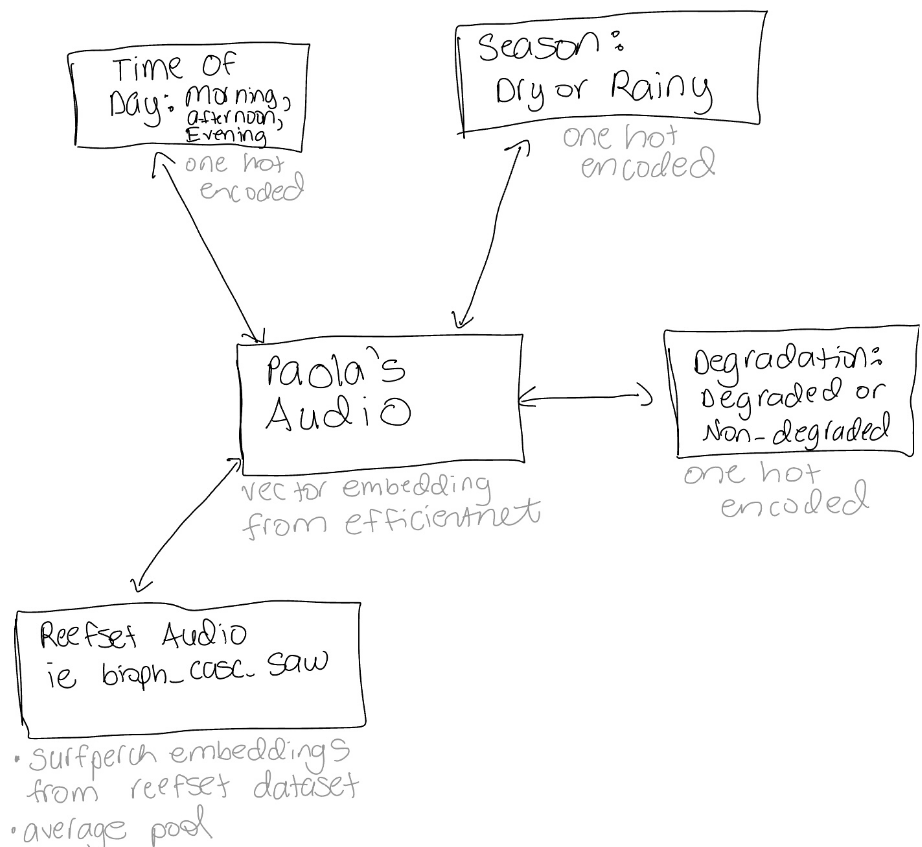
\includegraphics[height=0.8\textheight,width=0.8\textwidth,keepaspectratio]{images/knowledge_graph.png}
        \end{column}
    \end{columns}
\end{frame}

\begin{frame}{Regression - Chi-Square Tests}
    \begin{itemize}
        \item 
    \end{itemize}
\end{frame}

\begin{frame}{Template Matching}
    \begin{itemize}
        \item 
    \end{itemize}
\end{frame}

\begin{frame}{Binary Classifier}
    \begin{itemize}
        \item 
    \end{itemize}
\end{frame}

\begin{frame}{Site Separation}
    \begin{itemize}
        \item 
    \end{itemize}
\end{frame}

\begin{frame}{D3.JS Visualization}
    \begin{itemize}
        \item 
    \end{itemize}
\end{frame}

\begin{frame}{Autoencoders - Both Teams}
    \begin{itemize}
        \item 
    \end{itemize}
\end{frame}

\begin{frame}{Collar Team Agenda}
    \begin{itemize}
        \item 
    \end{itemize}
\end{frame}